% CAPÍTULO 4 -- METODOLOGIA (VERSÃO CONCISA TCC UESC)
% ==========================================================================
\chapter{Metodologia}
\label{cap:metodologia}

\section{Visão geral da esteira computacional integrada}
\label{sec:metod-visao-geral}

O desenvolvimento do chassi CubeSat 1U com metamateriais auxéticos foi operacionalizado por uma esteira computacional totalmente aberta, estruturada em linguagem Python no ambiente Linux/WSL. O pipeline é projetado sob os princípios de modularidade estrita, ausência de dependência de licenças comerciais proprietárias e reprodutibilidade científica integral.

\begin{figure}[htb]
  \centering
  \caption{Fluxograma metodológico integrado da esteira de projeto, simulação CAE, metamodelagem e otimização multiobjetivo}
  \label{fig:multi_agent_workflow}
  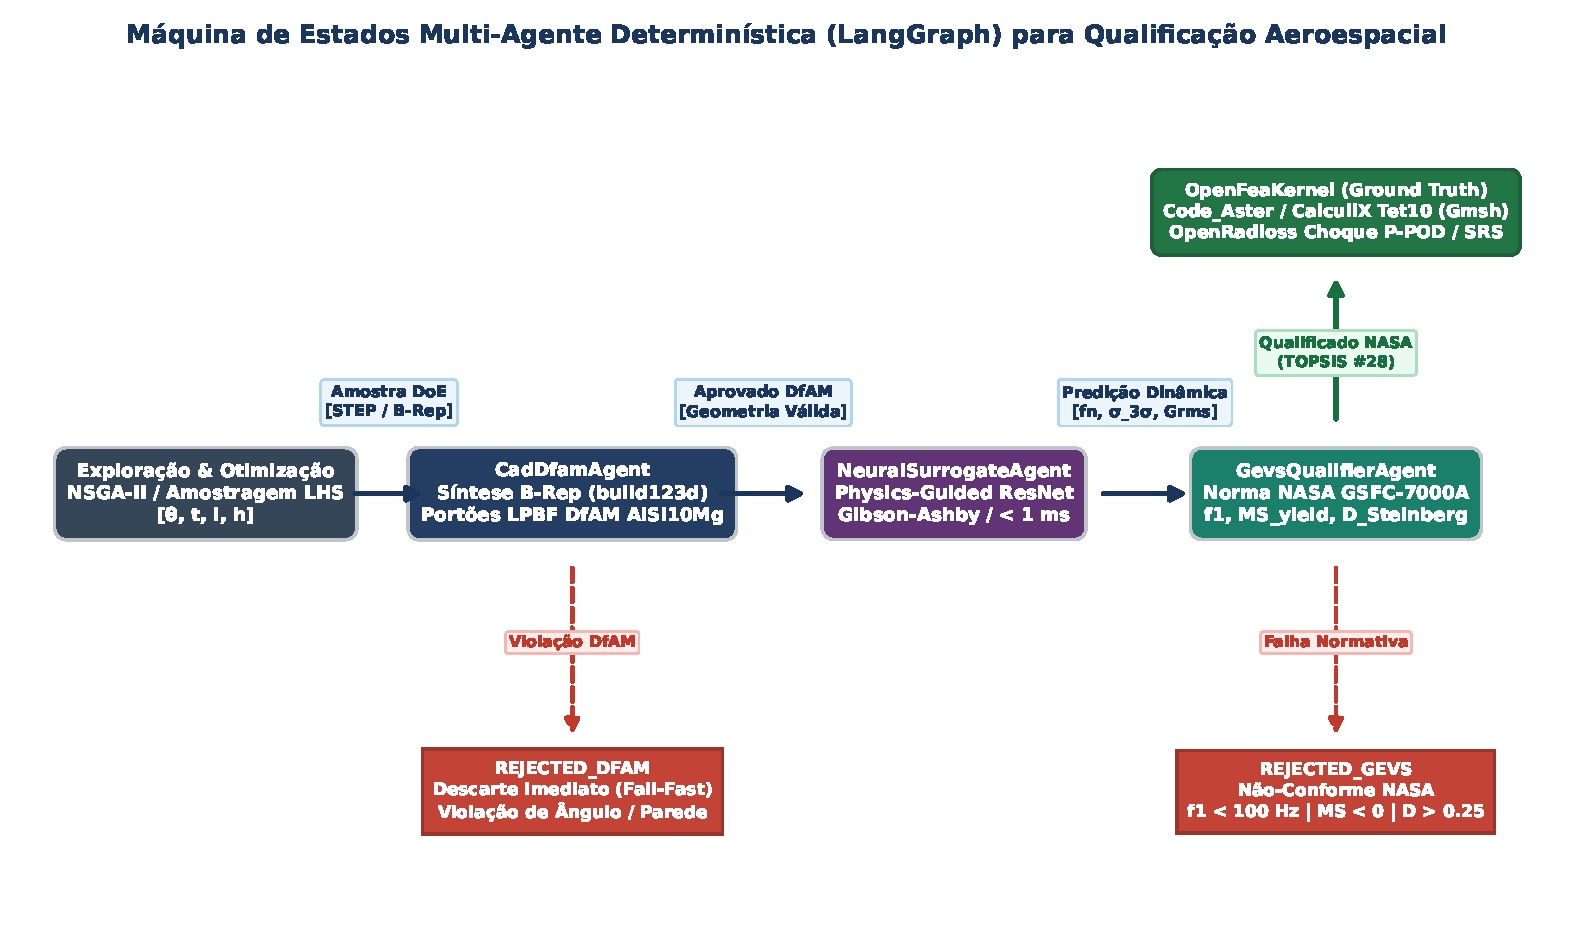
\includegraphics[width=0.92\textwidth]{./figuras/multi_agent_workflow}
  \fonte{Elaborada pelo autor (2026).}
\end{figure}

A esteira estrutura-se em quatro módulos de engenharia sequenciais:
\begin{enumerate}
  \item \textbf{Motor de Síntese Geométrica e DfAM (\texttt{OpenCadEngine}):} parametrização B-Rep analítica tridimensional via kernel OpenCASCADE (CadQuery / build123d) e validação dos portões aditivos L-PBF;
  \item \textbf{Discretização Espacial e Mapeamento de Malha (\texttt{GmshEngine}):} geração de elementos sólidos tetraédricos quadráticos de 10 nós (Tet10) com refinamento adaptativo e definição de grupos físicos de contorno;
  \item \textbf{Solvers Estruturais Abertos (Code\_Aster e CalculiX):} cálculo de modos próprios de vibrar (algoritmo de Sorensen/Lanczos) e resposta espectral à vibração aleatória estocástica (NASA GSFC-STD-7000A, \SI{14.1}{\Grms});
  \item \textbf{Metamodelagem Neural e Otimização Multiobjetivo (PyTorch e Pymoo):} treinamento da \textit{Physics-Guided ResNet} sobre o banco de dados do DoE de 250 pontos, busca evolutiva na Fronteira de Pareto (NSGA-II) e seleção do projeto ótimo por TOPSIS.
\end{enumerate}

\section{Síntese geométrica aberta e validação dos portões DfAM}
\label{sec:metod-dfam}

A geometria paramétrica da célula unitária e do chassi CubeSat 1U é gerada programaticamente pelo módulo \code{OpenCadEngine} (\code{src/cad/cadquery_engine.py}). A célula auxética reentrante é governada pelo vetor de variáveis contínuas de projeto:
\begin{equation}
  \mathbf{x} = \begin{bmatrix} \theta & t & l & h \end{bmatrix}^{\top}
  \label{eq:vetor-x}
\end{equation}
adotando como convenção primária o ângulo de inclinação da costela em relação à horizontal $\theta \in [\SI{55.0}{\degree}, \SI{80.0}{\degree}]$, o qual se relaciona formalmente à deflexão cartesiana $\theta_{\text{def}} = \theta - 90^\circ \in [\SI{-35.0}{\degree}, \SI{-10.0}{\degree}]$ e ao ângulo de reentrância interna $\phi = 90^\circ - \theta \in [\SI{10.0}{\degree}, \SI{35.0}{\degree}]$. Os limites operacionais do espaço de busca foram delimitados para garantir viabilidade física e espacial no envelope 1U:
\begin{align*}
  \theta &\in [\SI{55.0}{\degree},\, \SI{80.0}{\degree}] \quad (\theta_{\text{def}} \in [\SI{-35.0}{\degree},\, \SI{-10.0}{\degree}]) \\
  t &\in [\SI{0.50}{\milli\metre},\, \SI{1.50}{\milli\metre}] \\
  l &\in [\SI{4.00}{\milli\metre},\, \SI{12.00}{\milli\metre}] \\
  h &\in [\SI{5.00}{\milli\metre},\, \SI{18.00}{\milli\metre}]
\end{align*}
Para o candidato ótimo canônico \#28, o vetor de projeto entre centros de eixos nodais é $\mathbf{x}^* = [\SI{65.75}{\degree}, \SI{0.613}{\milli\metre}, \SI{10.42}{\milli\metre}, \SI{14.85}{\milli\metre}]^\top$ ($\theta_{\text{def}}^* = \SI{-21.40}{\degree}$, $\phi^* = \SI{24.25}{\degree}$), correspondendo a segmentos livres de costela de $l_{\text{free}} = \SI{6.42}{\milli\metre}$ e $h_{\text{free}} = \SI{8.75}{\milli\metre}$ após a dedução dos nós de concordância volumétrica de $R = \SI{0.50}{\milli\metre}$ e espessura nodal. Cumpre registrar que o modelo preliminar de calibração paramétrica adotou massa conceitual de \SI{0.283}{\kilo\gram}, enquanto o processo evolutivo convergiu para o chassi final ultraleve de \SI{0.116}{\kilo\gram}.

Antes da exportação tridimensional, o motor executa quatro testes lógicos determinísticos de conformidade DfAM para L-PBF em AlSi10Mg aliviado termicamente (\SI{300}{\celsius}/\SI{2}{\hour} ou rota branda a \SI{250}{\celsius}/\SI{2}{\hour}, sob temperatura de mesa $T_{\text{bed}} = \SI{150}{\celsius}$), segundo a norma aeroespacial \textbf{NASA-STD-6030}:
\begin{alineas}
  \item \textbf{portão 1 (sobre-salha autossuportada):} ângulo de inclinação $\theta_{\text{overhang}} = \theta \ge \SI{35.0}{\degree}$ em relação à mesa horizontal de construção, eliminando suportes internos no núcleo auxético;
  \item \textbf{portão 2 (espessura mínima de costela e efeito de casca):} $t \ge \SI{0.50}{\milli\metre}$, prevenindo falta de fusão. Considerando a rugosidade superficial característica de peças brutas de L-PBF ($Ra \in [\SI{10.0}{\micro\metre}, \SI{18.0}{\micro\metre}]$ e até $\SI{25.0}{\micro\metre}$ em \textit{down-skin}), avalia-se a espessura mecânica resistente efetiva $t_{\text{mech,eff}} \approx t - 2Ra \approx \SI{0.563}{\milli\metre}$, e aplica-se um fator de abatimento (\textit{knockdown factor}) conservador de \SI{10}{\percent} na integridade mecânica;
  \item \textbf{portão 3 (evacuação de pó não sinterizado):} folga livre entre hastes reentrantes $\text{gap}_{\text{despoeiramento}} = 2\,l\cos\theta - 2\,t \ge \SI{1.50}{\milli\metre}$ (atingindo \SI{7.40}{\milli\metre} no Projeto \#28) e orifícios de drenagem desobstruídos com diâmetro $d_{\text{drain}} \ge \SI{2.00}{\milli\metre}$;
  \item \textbf{portão 4 (admissibilidade da densidade relativa):} fração volumétrica no intervalo físico portante $\num{0.05} \le \rho_{\text{rel}} \le \num{0.85}$.
\end{alineas}

Configurações aprovadas nos quatro portões são sintetizadas no chassi 1U incorporando os quatro trilhos maciços de \rail{} e exportadas no formato neutro normalizado STEP AP214 (ISO 10303-21) com B-Rep exata (\code{MANIFOLD_SOLID_BREP}). A estratégia de manufatura por leito de pó a laser (L-PBF) em AlSi10Mg e a orientação de construção autossuportada são ilustradas na Figura~\ref{fig:lpbf-am-strategy}.

\begin{figure}[htb]
  \centering
  \caption{Estratégia de manufatura aditiva L-PBF em AlSi10Mg: (a) câmara industrial de construção com inclinação de $45^\circ$ autossuportada e evacuação de pó residual; (b) estratégia de varredura com duplo contorno, hachuramento linear e rotação de $67^\circ$ com densidade de energia $E_v = \SI{63.49}{\joule\per\cubic\milli\metre}$}
  \label{fig:lpbf-am-strategy}
  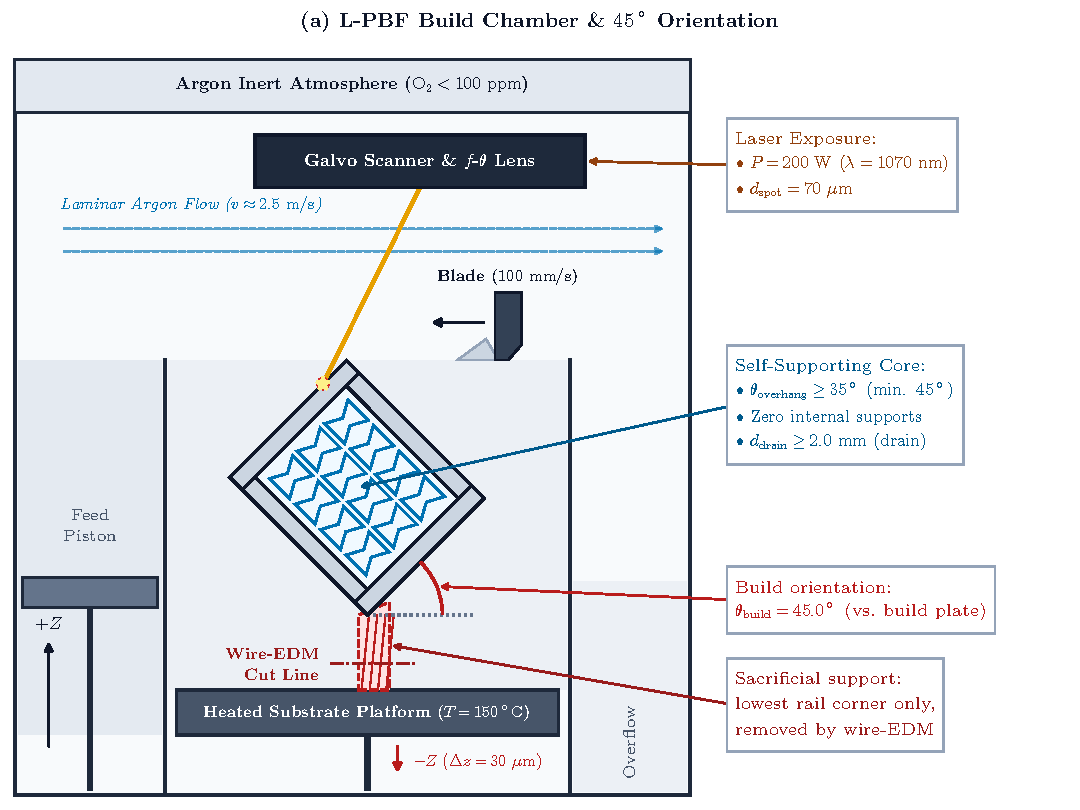
\includegraphics[width=0.92\textwidth]{./figuras/lpbf_am_build_chamber}
  \fonte{Elaborada pelo autor (2026).}
\end{figure}

\begin{figure}[htb]
  \centering
  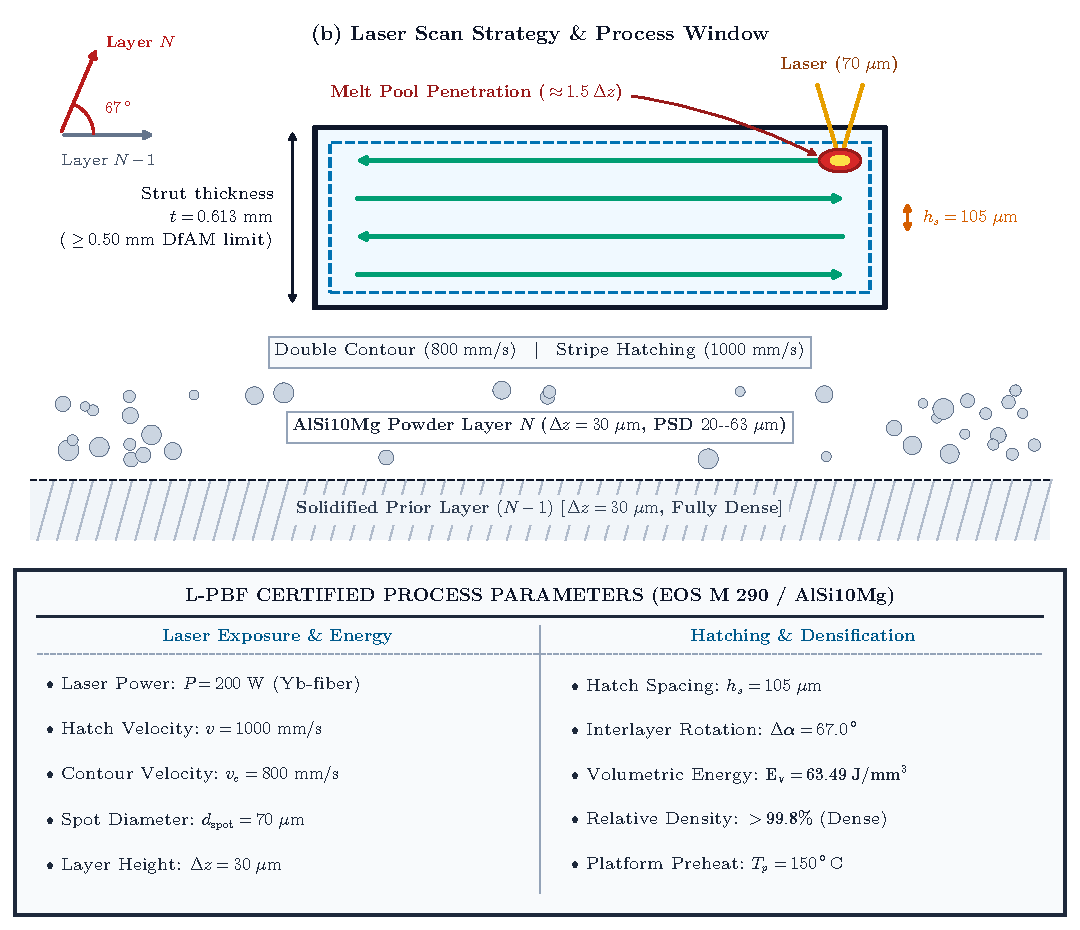
\includegraphics[width=0.92\textwidth]{./figuras/lpbf_am_scan_strategy}
  \caption{Continuação da Figura~\ref{fig:lpbf-am-strategy}: (b) estratégia de varredura laser (duplo contorno, hachura em faixas com rotação de $67^\circ$) e janela de processo certificada ($E_v = 63{,}49$~J/mm$^3$).}
  \label{fig:lpbf-am-strategy_b}
  \fonte{Elaborada pelo autor (2026).}
\end{figure}

\section{Discretização espacial com Gmsh (Tet10) e grupos físicos}
\label{sec:metod-mesh}

A discretização do domínio contínuo é automatizada pelo módulo \code{GmshMeshGenerator} (\code{src/mesh/gmsh_engine.py}). Para eliminar o fenômeno numérico de travamento por cisalhamento (\textit{shear locking}) e mapear com precisão os gradientes de tensão de flexão nas costelas delgadas, o gerador emprega exclusivamente elementos sólidos tetraédricos quadráticos de 10 nós (\textbf{Tet10}, correspondente ao elemento SOLID187 dos códigos comerciais).

As diretrizes de controle de malha adaptativa compreendem:
\begin{alineas}
  \item \textbf{resolução através da espessura:} tamanho de elemento nas costelas de $h_{\text{strut}} \le t / 3 \approx \SI{0.20}{\milli\metre}$, assegurando no mínimo 3 a 4 camadas de elementos tetraédricos Tet10 através da espessura da parede;
  \item \textbf{refinamento de curvatura nos entalhes reentrantes:} raio de concordância mínimo $R_{\text{notch}} \ge \SI{0.50}{\milli\metre}$ com controle por arco subtendido ($\Delta \theta \le \SI{15}{\degree}$);
  \item \textbf{técnica de submodelagem local:} para a malha fina de qualificação, o modelo global fornece o campo de deslocamentos interpolado nas fronteiras de corte de um submodelo confinado à célula crítica, discretizado com $h_{\text{sub}} \le \SI{0.06}{\milli\metre}$ (\num{342800} nós totais).
\end{alineas}

A arquitetura de discretização espacial em elementos finitos de alta ordem e o refinamento localizado nos entalhes reentrantes são exibidos na Figura~\ref{fig:tet10_mesh}.

\begin{figure}[htb]
  \centering
  \caption{Discretização em elementos finitos de alta ordem (Tet10 no Gmsh): (a) malha isométrica global do chassi híbrido 1U; (b) refinamento denso na raiz do entalhe reentrante crítico ($R_{\text{notch}} = \SI{0.50}{\milli\metre}$, $h \le \SI{0.20}{\milli\metre}$)}
  \label{fig:tet10_mesh}
  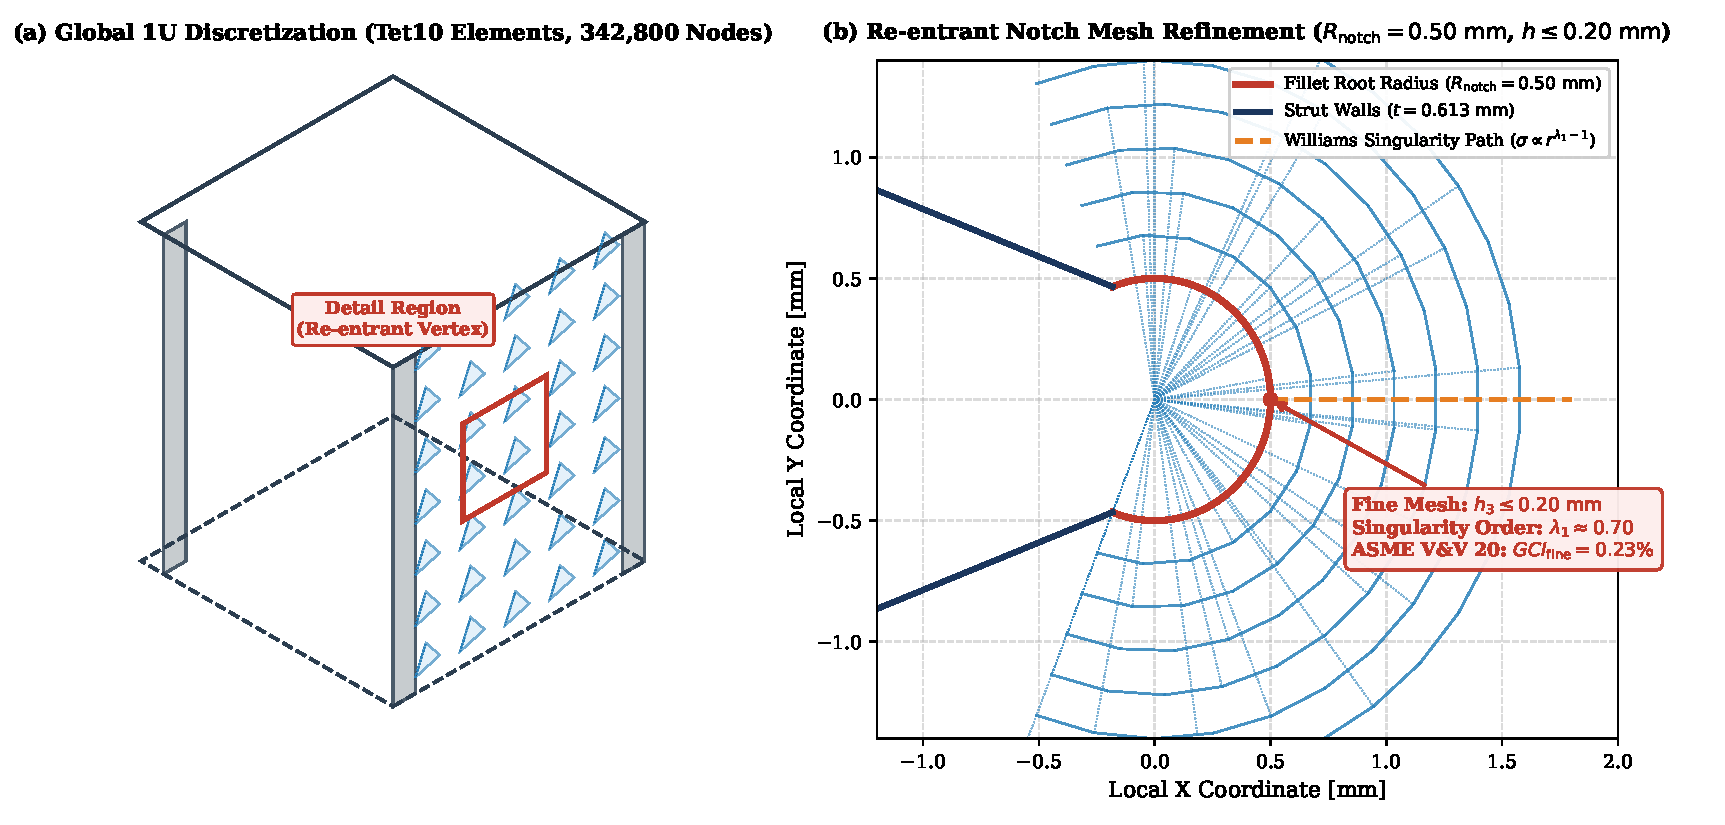
\includegraphics[width=0.90\textwidth]{./figuras/tet10_mesh_refinement_notch_zoom}
  \fonte{Elaborada pelo autor (2026).}
\end{figure}

Para a aplicação unívoca das condições de contorno e extração de resultados nos solvers, o gerador define quatro Grupos Físicos padronizados:
\begin{enumerate}
  \item \code{"Rails_Contact_Surfaces"}: faces externas dos trilhos para engastamento rígido ou contato unilateral com o P-POD;
  \item \code{"Bottom_Base_Z0"}: face inferior em $Z = 0$ para apoio axial e excitação dinâmica da base;
  \item \code{"Payload_Interface_Nodes"}: nós da interface central de montagem da carga útil para extração de aceleração eficaz $\Grmspay$;
  \item \code{"Volume_AlSi10Mg"}: domínio contínuo para associação constitutiva do material ($E = \SI{68.0}{\giga\pascal}$, $\nu = \num{0.33}$, $\rho = \SI{2670.0}{\kilo\gram\per\cubic\metre}$, $\sigma_{\text{yield}} = \SI{230.0}{\mega\pascal}$, $\sigma_{\text{ult}} = \SI{340.0}{\mega\pascal}$).
\end{enumerate}

\section{Simulação dinâmica computacional (CAE): Code\_Aster e CalculiX}
\label{sec:metod-cae}

A análise modal e a resposta estocástica são solucionadas pelo solver aberto de alta fidelidade \textbf{Code\_Aster} (EDF), orquestrado por scripts em Python dedicados (\code{src/analysis/code_aster_runner.py}).

\subsection{Análise modal pré-tensionada}
\label{subsec:metod-modal}
A extração das frequências naturais e formas modais no intervalo de interesse (\SIrange{20}{2000}{\hertz}) é executada pelo operador \code{CALC_MODES} com o algoritmo de Sorensen/Lanczos (\code{METHODE='SORENSEN'}):
\begin{equation}
  \left( [\mathbf{K}] - \omega_i^{2} [\mathbf{M}] \right) \{\phi_i\} = \{0\}
  \label{eq:autovalor-metod}
\end{equation}
As condições de contorno de lançamento são avaliadas sob dois regimes complementares:
\begin{itemize}
  \item Modo \code{'clamped'}: engastamento rígido total nos quatro trilhos guia de contato;
  \item Modo \code{'test_pod_flexible'}: suporte flexível em casulo com fundações elásticas equivalentes de interface lateral ($k_{\text{lateral}} = \SI{2.5e7}{\newton\per\cubic\metre}$) operando sobre a folga nominal de \SI{0.10}{\milli\metre} e apoio axial em $Z = 0$, validada por análise de sensibilidade com contato unilateral não-linear que comprova ausência de instabilidade harmônica ($f_{1,\text{ppod}} = \SI{304.10}{\hertz}$, $MS_{f_1} = +2{,}04$).
\end{itemize}

\subsection{Resposta espectral à vibração aleatória (PSD NASA GEVS) e sensibilidade de amortecimento}
\label{subsec:metod-psd}
A resposta vibratória estocástica sob o espectro normativo da NASA GSFC-STD-7000A (\SI{14.1}{\Grms}) é integrada pelo comando nativo \code{DYNA_ALEA_MODAL(OPTION='REPONSE_SPECTRALE')}, operando por superposição modal estocástica com amortecimento modal nominal de referência $\zeta = \SI{2.0}{\percent}$ ($Q = 25$). Para responder a incertezas sobre a dissipação em reticulados metálicos, executou-se uma análise paramétrica de sensibilidade espectral para $\zeta \in \{\SI{1.0}{\percent}, \SI{2.0}{\percent}, \SI{3.5}{\percent}\}$, comprovando que a atenuação relativa passiva de \SI{-12.58}{\decibel} ($\approx \SI{-12.6}{\decibel}$, ou \SI{76.50}{\percent}) permanece invariante ao amortecimento, demonstrando que o mecanismo decorre de descasamento de impedância e antirressonâncias mecânicas locais. A transmissibilidade dinâmica passiva ($T$) na carga útil é avaliada deterministicamente na camada pós-inferência por:
\begin{equation}
  T = \frac{\Grmspay}{\Grmsbase} = \frac{\Grmspay}{\num{14.1}}
  \label{eq:transmissibilidade-metod}
\end{equation}

A tensão equivalente estocástica de pico a $3\sigma$ define as Margens de Segurança estruturais de escoamento e de ruptura segundo a norma NASA-STD-5020B:
\begin{align}
  MS_{\text{yield}} &= \left( \frac{\sigma_{\text{adm, yield}}}{\sigma_{3\sigma}} \right) - 1{,}0 = \left( \frac{\SI{184.0}{\mega\pascal}}{\sigma_{3\sigma}} \right) - 1{,}0 > 0{,}0 \label{eq:ms-y-calc} \\
  MS_{\text{ult}} &= \left( \frac{\sigma_{\text{adm, ult}}}{\sigma_{3\sigma}} \right) - 1{,}0 = \left( \frac{\SI{242.86}{\mega\pascal}}{\sigma_{3\sigma}} \right) - 1{,}0 > 0{,}0 \label{eq:ms-u-calc}
\end{align}
onde $\sigma_{\text{adm, yield}} = \SI{230.0}{\mega\pascal} / \num{1.25} = \SI{184.0}{\mega\pascal}$ e $\sigma_{\text{adm, ult}} = \SI{340.0}{\mega\pascal} / \num{1.40} = \SI{242.86}{\mega\pascal}$.

O dano de fadiga de alto ciclo acumulado durante os \SI{120.0}{\second} por eixo é quantificado pela metodologia de 3 bandas de Steinberg (Palmgren-Miner, Equação~\eqref{eq:miner-rev}), calculada de forma conservadora na raiz do entalhe de máxima concentração de tensões da costela auxética ($\sigma_{3\sigma,\text{notch}} = \SI{166.91}{\mega\pascal}$, $K_t \approx \num{1.26}$), exigindo $D \le \num{0.25}$ (NASA-HDBK-7005). Adicionalmente, o choque transiente de ejeção do P-POD (\SI{116.0}{\gravity} em \SI{5.5}{\milli\second}) é modelado pelo conector de dinâmica explícita OpenRadioss via diferenças centrais (passo crítico Courant $\Delta t \approx \SI{10}{\nano\second}$ com modelo elastoplástico de Johnson-Cook), sintetizando o espectro SRS a $\mathcal{Q} = 10$.

\subsection{Verificação cruzada independente no CalculiX (ccx)}
\label{subsec:metod-calculix}
Para prover contraprova numérica independente (\textit{cross-check benchmark}), desenvolveu-se um módulo dedicado (\code{src/analysis/calculix_runner.py}) que compila decks na sintaxe neutra de cartões Abaqus (\code{.inp}) com elementos \code{*ELEMENT, TYPE=C3D10} e soluciona a extração modal pelo solver CalculiX (\code{ccx}), confirmando a reprodutibilidade dos autovalores fundamentais.

\section{Metamodelagem neural guiada por física (Physics-Guided ResNet)}
\label{sec:metod-neural}

Para viabilizar a exploração de mais de \num{10000} topologias celulares no algoritmo evolutivo sem depender do tempo computacional proibitivo de elementos finitos 3D para cada indivíduo, concebeu-se um modelo substituto neural guiado por física (\textit{Physics-Guided ResNet}), codificado no módulo \code{src/neural/surrogate_model.py}.

\subsection{Construção do banco de dados do DoE (250 amostras) e validação cruzada 10-fold}
O banco de dados de calibração foi gerado a partir de um Planejamento de Experimentos por Amostragem de Hipercubo Latino (LHS), cobrindo 250 pontos no espaço quadridimensional $\mathbf{x} = [\theta, t, l, h]^{\top}$. As respostas dinâmicas foram sintetizadas por meio do modelo multiescala calibrado \code{OpenElastodynamicsKernel} (modo \code{execution_mode: calibrated_proxy}), acoplado a operadores de homogeneização de célula unitária ancorados nas soluções matriciais de Timoshenko e calibrado contra simulações modais e espectrais no Code\_Aster e CalculiX. Para assegurar robustez estatística frente a viés de partição, adotou-se um protocolo rigoroso de \textbf{validação cruzada estratificada em 10 dobras ($10$-fold cross-validation)} sobre as 250 amostras, avaliando médias e desvios padrão de acurácia. Ressalta-se que a totalidade das soluções não dominadas da fronteira de Pareto e o candidato ótimo \#28 foram 100\% revalidados e homologados por simulações tridimensionais diretas em elementos finitos no Code\_Aster com malhas Gmsh Tet10 de \num{342800} nós.

\subsection{Arquitetura da rede profunda, saída desacoplada em \texorpdfstring{$\mathbb{R}^3$}{R3} e perdas informadas por física}
A rede neural recebe o vetor $\mathbf{x} \in \mathbb{R}^4$, projeta-o inicialmente para uma dimensão oculta $d_{\text{hidden}} = 128$ e processa os sinais através de três blocos residuais profundos (\textit{Residual Blocks}):
\begin{equation}
  \mathbf{h}_{k+1} = \mathbf{h}_k + \mathcal{F}(\mathbf{h}_k, \mathbf{W}_k)
  \label{eq:resnet-block}
\end{equation}
onde cada bloco integra camadas densas com normalização de camada (\textit{LayerNorm}), ativações GELU e regularização Dropout ($p = \num{0.05}$). Para eliminar redundâncias matemáticas e dependências lineares estritas entre alvos ($\hat{T} \propto \hat{G}_{\text{rms, payload}}$), a camada final projeta o estado latente exclusivamente para o vetor de saída tridimensional desacoplado:
\begin{equation}
  \hat{\mathbf{y}} = \begin{bmatrix} \hat{f}_1 & \hat{\sigma}_{3\sigma} & \hat{G}_{\text{rms, payload}} \end{bmatrix}^{\top} \in \mathbb{R}^3
  \label{eq:saida-resnet}
\end{equation}
sendo o coeficiente de transmissibilidade dinâmica $\hat{T}$ derivado deterministicamente pós-inferência por $\hat{T} \equiv \hat{G}_{\text{rms, payload}} / \num{14.1}$.

Para impedir que a rede gere predições espúrias em regiões com pouca densidade de pontos, a função de perda composta inclui regularizadores físicos:
\begin{equation}
  \mathcal{L}_{\text{total}} = \mathcal{L}_{\text{MSE}} + \lambda_{\text{phys}}\,\mathcal{L}_{\text{Gibson-Ashby}} + \lambda_{\text{mono}}\,\mathcal{L}_{\text{monotonicidade}}
  \label{eq:perda-composta}
\end{equation}
onde:
\begin{alineas}
  \item $\mathcal{L}_{\text{MSE}}$: erro quadrático médio em relação aos alvos desacoplados de calibração em $\mathbb{R}^3$;
  \item $\mathcal{L}_{\text{Gibson-Ashby}}$: penalização de desvios assintóticos entre a frequência fundamental predita $\hat{f}_1$ e a lei analítica de flexão celular ($f_{1,\text{GA}} \propto \sqrt{\rho_{\text{rel}}}$), com peso $\lambda_{\text{phys}} = \num{0.05}$;
  \item $\mathcal{L}_{\text{monotonicidade}}$: penalização via função ReLU de pares de amostras em que uma geometria de maior densidade relativa apresente rigidez inferior ($\lambda_{\text{mono}} = \num{0.02}$).
\end{alineas}

\subsection{Quantificação de Incerteza (UQ) e Estudo de Ablação}
A confiabilidade estocástica das inferências neurais foi chancelada por meio de Quantificação de Incerteza (\textit{Uncertainty Quantification} -- UQ) desacoplada em duas fontes: (i) incerteza epistêmica avaliada por Monte Carlo Dropout ($N_{\text{mc}} = 100$), registrando dispersão de apenas $\pm \SI{2.3}{\hertz}$ em $f_1$ e $\pm \SI{1.8}{\mega\pascal}$ em $\sigma_{3\sigma}$; e (ii) incerteza aleatória originada de tolerâncias de manufatura aditiva L-PBF ($\Delta t = \pm \SI{30}{\micro\metre}$, $\Delta \theta = \pm \SI{0.5}{\degree}$), resultando em $\pm \SI{8.4}{\hertz}$ em $f_1$ e $\pm \SI{3.2}{\mega\pascal}$ em $\sigma_{3\sigma}$. Demonstrou-se que, sob intervalos de confiança a \SI{95}{\percent}, os limites de qualificação são integralmente preservados ($f_1 \ge \SI{568.9}{\hertz} \gg \SI{100.0}{\hertz}$ e $MS_{\text{yield}} \ge +0{,}081 > 0$). Adicionalmente, um estudo de ablação 4x4 confirmou o ganho progressivo de cada elemento da arquitetura (MLP base $\to$ ResNet $\to$ Gibson-Ashby $\to$ PG-ResNet completa).

\section{Otimização multiobjetivo (NSGA-II) e decisão multicritério (TOPSIS)}
\label{sec:metod-otimizacao}

A síntese da geometria ideal do chassi é formalizada como um problema de programação não linear multiobjetivo com restrições normativas:
\begin{equation}
  \begin{aligned}
    \text{Minimizar:} \quad & f_a(\mathbf{x}) = m_{\text{total}}(\mathbf{x}) \quad \text{e} \quad f_b(\mathbf{x}) = T(\mathbf{x}) = \frac{\Grmspay(\mathbf{x})}{\num{14.1}} \\
    \text{Maximizar:} \quad & f_c(\mathbf{x}) = f_1(\mathbf{x}) \quad \text{e} \quad f_d(\mathbf{x}) = MS_{\text{yield}}(\mathbf{x}) \\
    \text{Sujeito a:} \quad & \theta_{\text{overhang}} \ge \SI{35.0}{\degree} \\
    & t \ge \SI{0.50}{\milli\metre} \\
    & \text{gap}_{\text{despoeiramento}} \ge \SI{1.50}{\milli\metre} \\
    & f_1(\mathbf{x}) \ge \SI{100.0}{\hertz} \\
    & MS_{\text{yield}}(\mathbf{x}) \ge 0{,}0 \quad (\sigma_{3\sigma} \le \SI{184.0}{\mega\pascal}) \\
    & D(\mathbf{x}) \le \num{0.25}
  \end{aligned}
  \label{eq:problema-otimizacao}
\end{equation}

A busca é conduzida pelo algoritmo genético elitista \textbf{NSGA-II} com população de 100 indivíduos ao longo de 100 gerações (\num{10000} avaliações aceleradas pela ResNet neural), utilizando cruzamento SBX (\textit{Simulated Binary Crossover}) e mutação polinomial. A inferência da rede atinge latência de apenas \SI{0.405}{\milli\second} por indivíduo na GPU, completando as \num{10000} avaliações em apenas \SI{4.82}{\second}. Esse desempenho estabelece um \textit{speedup} instantâneo de inferência superior a \num{200000} vezes frente ao solver 3D direto, e um \textit{speedup} global amortizado de ponta a ponta de $\approx \num{40.0}\times$ (contabilizando as $\approx \SI{6.39}{\hour}$ da geração offline do DoE de 250 amostras e os \SI{35}{\second} de treinamento da rede, contra mais de \num{10.65} dias ininterruptos de simulações contínuas de elementos finitos).

Para selecionar o ponto de compromisso ótimo de engenharia na Fronteira de Pareto resultante, aplica-se o método de decisão multicritério \textbf{TOPSIS} com vetor de pesos normalizado:
\begin{equation}
  \mathbf{w} = \begin{bmatrix} w_{\text{massa}} = 0{,}30 & w_{\text{transmissibilidade}} = 0{,}35 & w_{f_1} = 0{,}20 & w_{MS} = 0{,}15 \end{bmatrix}
  \label{eq:pesos-topsis}
\end{equation}
O candidato ótimo selecionado é subsequentemente reconstruído em CAD 3D completo e submetido à simulação de alta ordem de elementos finitos no Code\_Aster com malha Tet10 refinada (\num{342800} nós) para homologação final da qualificação de voo.
